
Рейтинг системы широко распространены в спортивных, киберспортивных и интеллектуальных соревнованиях.
Они используются для подбора соперников по уровню.


Рейтинг-система – это модель, которая ранжирует
участников (игроков) в единый линейный порядок по
данным сравнений небольших подмножеств этих игроков
(турниров)
 
В этом случае рейтинг можно задать как оператор $\zeta$ принимающий на вход потенциалы, задающие силу объекта.
\begin{equation}
    p(x_i \succ x_j) = \zeta(\phi(x_i),\phi(x_j))
\end{equation}
Согласно модели рейтинга Эло сила игрока задается случайной величиной $\xi$. 
Экспоненциальный вид графика связан с предположением о том, что в стратегических играх существенное различие в навыке гарантирует победу
\textit{Рейтинг} задается матожиданием силы $\mathcal{E} \xi$.
Согласно модели Эло сила игрока задается нормально, причем дисперсия $\sigma$ фиксирована для всех игроков
Тогда сила игры согласно предположению определяется как:
\begin{equation}
    p(x) = \frac{1}{\sigma \sqrt{2\pi}} \exp^{- \frac{1}{2\sigma^2}{(x-s)^2}}
\end{equation}
Таким образом, рейтинг является латентной переменной. В литературе также популярна модель Брэдли-Терри,задающая
вероятность победы зависит как:
\begin{equation}
    P(\theta)
\end{equation}
Заметим, что подмена $\gamma ~ exp(-\theta/\beta^2)$ позволяет отождествить подходы.
В шахматной практике волатильность считается определенной и имеет стандартное отклонение равное 20:
\begin{equation}
    \frac{1}{1+10^\frac{R_B-R_A}{400}} 
\end{equation}

\begin{figure}[h]
    \centering
    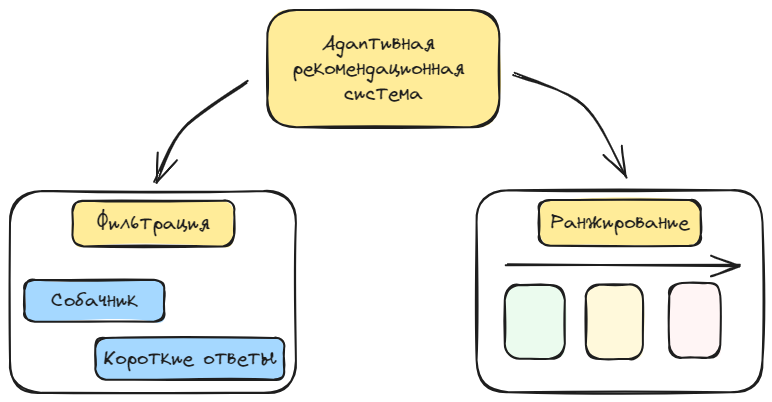
\includegraphics[width=0.5\textwidth]{assets/work/rating/bayes.excalidraw.png}
    \caption{Устройство байесового пересчета }
    \label{bayes}
\end{figure}

\textit{Лемма} Модель является игрой с нулевой суммой. 

\texit{Доказательство} Правило обновления


\textit{Лемма} Рейтинг Эло является устойчивым. В отсутствие изменений силы игрока в ходе обновлений рейтинга оценка станет истинной

\texit{Доказательство} Используем переход к модели Брэдлли-Терри.

Существуют также модель, учитывающие занятие одинаковой позиции в ступень ранга \cite{plackett1975analysis}\cite{luce2005individual}. 
Минус подходы заключается в вычислительной сложности пересчета.